\section{Transformée de Fourier quantique (QFT)}
La QFT est l'équivalent quantique de la DFT inverse à cause de certaines conventions de signes \cite{nielsen00}. Ainsi, on travaille avec des bras/kets dans un espace de Hilbert de dimension $N= 2^n$ où $n$ est le nombre de qubits. On regarde son effet sur un vecteur de base $\ket*{j}$ en gardant en tête que $k = \sum_{l=0}^{n-1}k_l 2^{l}$ est la représentation binaire de $k$ où $k_l \in \{0,1\}$.

\begin{equation*}
    \text{QFT}\ket*{j} = \frac{1}{\sqrt{N}}\sum_{k=0}^{N-1}e^{\frac{2\pi i}{N}jk}\ket*{k} = \frac{1}{\sqrt{N}}\sum_{k_{n-1} = 0}^{1} ... \sum_{k_0 = 0}^{1}e^{2\pi i j\sum_{l=0}^{n-1}k_l \frac{2^{l}}{2^n}}\ket*{k_{n-1} ... k_{0}}
\end{equation*}

\begin{equation*}
    = \frac{1}{\sqrt{N}}\sum_{k_{n-1} = 0}^{1} ... \sum_{k_0 = 0}^{1} e^{2\pi i j \sum_{l=0}^{n-1} \frac{k_l}{2^{n-l}}} \ket*{k_{n-1} ... k_{0}} = \frac{1}{\sqrt{N}}\sum_{k_{n-1} = 0}^{1} ... \sum_{k_0 = 0}^{1} \prod_{l=0}^{n-1} e^{2\pi i j \frac{k_l}{2^{n-l}}} \ket*{k_{n-1}} \otimes ... \otimes \ket*{k_{0}}
\end{equation*}

Par convention, on voudrait plutôt que l'ordre du produit soit inversé, ce qu'on fait en changeant $2^{n-l}$ par $2^{l+1}$. Ainsi, 
\begin{equation*}
    \frac{1}{\sqrt{N}}\sum_{k_{n-1} = 0}^{1} ... \sum_{k_0 = 0}^{1} \prod_{l=0}^{n-1} e^{2\pi i j \frac{k_l}{2^{l+1}}} \ket*{k_{n-1}} \otimes ... \otimes \ket*{k_{0}} = \frac{1}{\sqrt{N}} \left( \sum_{k_{n-1} = 0}^{1} e^{2\pi i j \frac{k_{n-1}}{2^n}} \ket*{k_{n-1}} \otimes ... \otimes \sum_{k_{0} = 0}^{1} e^{2\pi i j \frac{k_{0}}{2}} \ket*{k_{0}}\right)
\end{equation*}

\begin{equation*}
    = \frac{1}{\sqrt{N}} \left[\left(\ket*{0} + e^{2\pi i\frac{j}{2^n}}\ket*{1} \right) \otimes ... \otimes \left(\ket*{0} + e^{2\pi i\frac{j}{2}}\ket*{1}\right)\right] = \frac{1}{\sqrt{N}}\bigotimes_{l=0}^{n-1} \left(\ket*{0} + e^{2\pi i \frac{j}{2^{l+1}}}\ket*{1}\right)
\end{equation*}

Comme $j$ est un entier qu'on pourrait représenter en binaire par $j = j_{n-1}...j_0$, alors $\frac{j}{2^{l+1}}$ décale les bits de $j$ vers la droite par $l+1$ positions. On aurait donc $\frac{j}{2^{l+1}} = j_{n-1}...j_{l+1}\pmb{.}j_l...j_0$ où le point sépare la partie entière (à gauche) de la partie fractionnaire (à droite). Par contre, puisque cette quantité se trouve dans une exponentielle complexe, la partie entière n'a aucun impact sur le calcul. De ce fait, on peut simplement garder la partie fractionnaire $0\pmb{.}j_l...j_0$ dans l'exponentielle. La notation $0\pmb{.}j_l ... j_0$ équivaut à $j_l2^{-1} + ... + j_0 2^{-(l+1)}$ et correspond à l'écriture en binaire d'un nombre décimal.  On a alors la forme finale de la QFT :

\begin{equation}
    \ket*{\phi(j)} = \text{QFT}\ket*{j} = \frac{1}{\sqrt{N}} \bigotimes_{l=0}^{n-1}\left(\ket*{0} + e^{2\pi i \ 0\pmb{.}j_l ... j_0} \ket*{1}\right) 
\end{equation}

où chaque qubit $\ket*{j_l}$ de l'état de base $\ket*{j}$ devient 

\begin{equation*}
    \ket*{\phi_l(j)} = \frac{1}{\sqrt{2}}\left(\ket*{0} + e^{2\pi i \ 0\pmb{.}j_l...j_0}\ket*{1}\right)
\end{equation*}

On cherche maintenant à construire le circuit permettant d'effectuer la QFT sur un état de base $\ket*{j}$, c'est-à-dire de trouver une implémentation équivalente à (5).
On utilisera la porte Hadamard $H$ et la porte de phase $R_k$.

\begin{equation*}
    R_k = \begin{bmatrix}
        1 & 0 \\
        0 & e^{2\pi i/2^k}
    \end{bmatrix}
\end{equation*}

L'application de $H$ sur $\ket*{j_{n-1}}$ entraîne l'ajout de  $j_{n-1}$ au début de l'exponentielle.

\begin{equation*}
    H\ket*{j_{n-1}} \ket*{j_{n-2} ... j_0} = \frac{1}{\sqrt{2}} \left(\ket*{0} + (-1)^{j_{n-1}} \ket*{1}\right) \ket*{j_{n-2} ... j_0} = \frac{1}{\sqrt{2}}\left(\ket*{0} + e^{2\pi i \ 0\pmb{.}j_{n-1}} \ket*{1} \right) \ket*{j_{n-2} ... j_0}
\end{equation*}

Puis, en appliquant $R_2$ contrôlée par $\ket*{j_{n-2}}$ sur le qubit de poids fort, on peut ajouter ce dernier  à l'exponentielle.  

\begin{equation*}
    CR_2 \left( \frac{1}{\sqrt{2}}\left(\ket*{0 j_{n-2}} + e^{2\pi i \ 0\pmb{.}j_{n-1}} \ket*{1 j_{n-2}} \right)\right) \ket*{j_{n-3} ... j_0} = \frac{1}{\sqrt{2}}\left(\ket*{0} + e^{2\pi i \ 0\pmb{.}j_{n-1}j_{n-2}} \ket*{1} \right) \ket*{j_{n-2} ... j_0}
\end{equation*}

En continuant ainsi de suite pour $CR_3, ..., CR_n$, on se retrouve avec

\begin{equation*}
    \frac{1}{\sqrt{2}} \left(\ket*{0} + e^{2\pi i \ 0\pmb{.}j_{n-1}...j_0} \ket*{1}\right) \ket*{j_{n-2} ... j_0}
\end{equation*}

ce qui correspond bien à l'état du dernier qubit de (5). Pour appliquer la QFT au complet, il suffit de suivre ce même principe pour chaque qubit de l'état de base $\ket*{j}$ afin d'obtenir globalement l'état correspondant à (5). Depuis ce circuit, il est par la suite facile d'obtenir QFT$^\dag$ qu'on nommera la QFT inverse.

\begin{figure}[H]
    \centering
    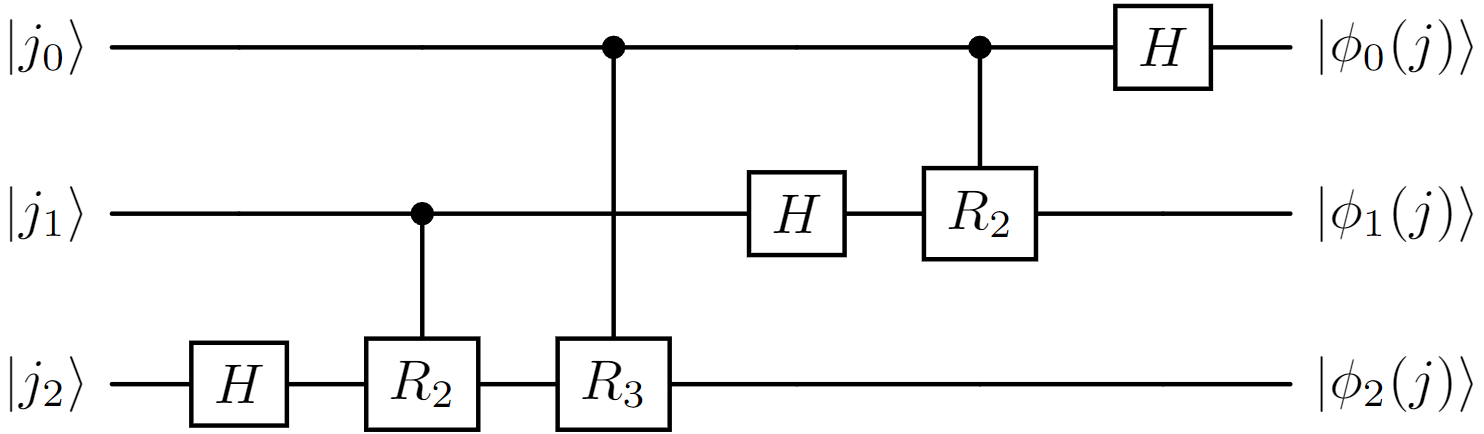
\includegraphics[scale=0.3]{images/circuit_qft.png} 
    \caption{Circuit de la QFT pour un état de base $\ket*{j}$ à 3 qubits}
\end{figure}

La QFT nécessite $n$ portes Hadamard et $\sum_{j=1}^{n}(n-j)$ portes de phase $\implies \mathcal{O}(n^2)$ où $n$ est le nombre de qubits. La FFT (analogue classique de la QFT) a une complexité $\mathcal{O}(Nlog(N)) = \mathcal{O}(2^n n)$. Il y a donc un avantage exponentielle à utiliser la QFT plutôt que la FFT. 